\begin{figure}[ht]
  \centerline{
    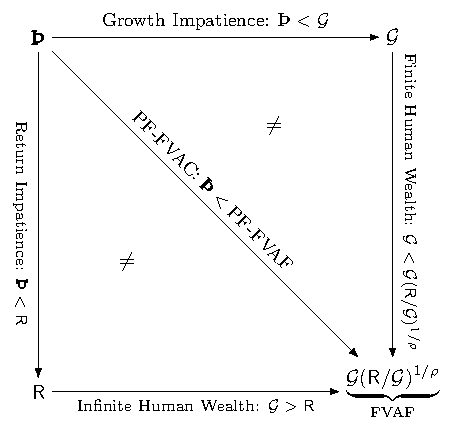
\includegraphics[width=3.5in]{\FigDir/RelatePFGICFHWCRICPFFVAC}
  }
  \caption{Perfect Foresight Relation of {GIC}, {FHWC}, {RIC}, and {PFFVAC}}
  \iflabelexists{fig:RelatePFGICFHWCRICPFFVAC}{}{\label{fig:RelatePFGICFHWCRICPFFVAC}} % Don't define it if already defined
  \footnotesize{An arrowhead points to the larger of the two quantities being compared.  For example, the diagonal arrow indicates that $\APFac < \Rfree^{1/\CRRA}\PermGroFac^{1-1/\CRRA}$, which is one way of writing the {\PFFVAC}, equation \eqref{eq:PFFVAC}}
\end{figure}
